\documentclass[11pt]{article}
\usepackage[margin=1in]{geometry}
\usepackage[T1]{fontenc}
\usepackage{lmodern}
\usepackage{microtype}
\usepackage{graphicx}
\usepackage{booktabs}
\usepackage{amsmath}
\usepackage[font=small,labelfont=bf]{caption}
\usepackage[numbers,sort&compress]{natbib}
\usepackage[hidelinks]{hyperref}
\usepackage{xurl}
\usepackage{xcolor}
\usepackage{enumitem}
\usepackage{tabularx}
\usepackage{float}
\usepackage[section]{placeins}
\setlist{itemsep=2pt,topsep=4pt}
\graphicspath{{../figures_v2/}}
\newcommand{\todo}[1]{\textcolor{orange}{[#1]}}
\newcolumntype{L}{>{\raggedright\arraybackslash}X}

\title{Chunked Prefill or Disaggregation?\\
\large Prefill--Decode Serving over TCP on Single-GPU Cloud Instances}
\author{Sunghyun Jun\\ Independent Researcher\\ \todo{contact email}}
\date{\todo{draft v2, 2026-10-01}}

\begin{document}
\maketitle

\begin{abstract}
Prefill--decode (PD) disaggregation usually relies on RDMA or NVLink, which the cheapest single-GPU cloud instances lack. We ask when disaggregation over TCP beats colocated replicas that use chunked prefill. On AWS 2xlarge instances we served Gemma~4 26B (mixture of experts) and 31B (dense) with stock vLLM, disaggregated with NIXL/UCX over TCP, and judged each request by its time to first token (TTFT) and its longest gap between output tokens. A replica stalls whenever another request's prefill shares its scheduler step, so the chunk size bounds that gap: for 26B with 4K-token inputs, the median fell from 48~ms at a 2,560-token chunk to 21~ms at 512. Under a 1~s TTFT and 50~ms gap limit, disaggregation served about 3$\times$ more requests per GPU than replicas held at 2,560 tokens, near the minimum vLLM allows Gemma~4 with video enabled. Against smaller chunks it never served more under any SLO we tested, down to 30~ms: for 26B it was borderline at 4 requests/s per GPU while replicas held 5; for 31B chat, 4 against at least 8. Its TTFT cost was mostly the KV transfer, which a larger UCX TCP segment made 3.4$\times$ faster. Tune the chunk first.
\end{abstract}

\section{Introduction}

Serving a request to a large language model takes two phases: \emph{prefill}, which processes the whole input at once, and \emph{decode}, which produces output tokens one at a time. When both share a GPU, a prefill scheduled into the same step as ongoing decodes lengthens that step, and every streaming request on that GPU pauses. Two remedies exist. \emph{Chunked prefill} splits a long prefill into pieces that are batched with decodes, which bounds the work any one step carries~\cite{sarathi2023,sarathi}. \emph{Disaggregation} runs the two phases on different GPUs and ships the KV cache from the prefill GPU to the decode GPU~\cite{distserve,splitwise,mooncake}.

Disaggregation pays for its isolation with a KV-cache transfer, and published systems run that transfer over fast links: InfiniBand~\cite{splitwise}, RDMA~\cite{mooncake}, or NVLink inside one node~\cite{distserve}. The cheapest single-GPU cloud instances offer none of these. On AWS, the 2xlarge sizes of the g6e, g7, and g7e families have one GPU, no Elastic Fabric Adapter (EFA), and no ENA Express~\cite{awsspecs}; the 8xlarge sizes of the same families add EFA at roughly 1.6--2$\times$ the hourly price~\cite{awsefa,vantage}. Public documentation discourages disaggregation over TCP: llm-d calls it ``extremely slow'' and ``targeted for local development''~\cite{llmddocs}, and NVIDIA Dynamo warns of a 200--500$\times$ slower TTFT without RDMA and recommends aggregated serving instead~\cite{dynamodocs}. Few public measurements show how slow the TCP path is, or whether disaggregation over it still beats a well-configured colocated deployment.

We measured both remedies on the same hardware. We served two Gemma~4 models with stock vLLM on one to three single-GPU instances, disaggregated them with vLLM's NIXL connector over UCX's TCP transport, and judged each request by its TTFT and by the longest gap between its output tokens. Our first comparison pitted disaggregation against replicas at the chunk size our stack first accepted. Two mock peer reviews of our drafts found that this baseline was handicapped twice: its chunk size was untuned, and its request proxy capped concurrent connections at 100. We added two sessions (E8 and E9) that swept the chunk size and removed the cap, and we committed our predictions for E9 before running it. These sessions changed the conclusion, and we report both baselines.

We ask three research questions (RQs):
\begin{itemize}
  \item \textbf{RQ1.} Under a per-request limit on the longest token gap, what sets the stalls of colocated replicas, and how far does chunked prefill go?
  \item \textbf{RQ2.} Over TCP, what does disaggregation cost in TTFT, and what determines that cost?
  \item \textbf{RQ3.} At equal GPU count, when does disaggregation over TCP serve more SLO-meeting load than tuned colocation?
\end{itemize}
In short: the chunk size sets the stall; the KV transfer sets disaggregation's TTFT cost; and in every SLO we tested, replicas with a tuned chunk served at least as much as disaggregation over TCP. Disaggregation won by about 3$\times$ only when the chunk was held near 2,500 tokens.

Our contributions are:
\begin{itemize}
  \item a joint evaluation of chunk size and disaggregation under per-request stall limits, with a map of where each wins as the SLO changes (Sections~\ref{sec:chunk}--\ref{sec:who});
  \item a characterization of the KV transfer over cloud TCP: the UCX segment size, NIXL's splitting of a transfer over up to four connections, the cloud's per-flow cap, and a KV-volume and TTFT model (Sections~\ref{sec:transfer}--\ref{sec:ttft});
  \item four pitfalls that changed our conclusions: percentile metrics hide per-request stalls; a multimodal budget check keeps Gemma~4's chunk at 2,496 tokens or more unless every modality is disabled; the reference proxy's garbage collection pauses all streams; and an HTTP client's default connection limit throttled the replicas (Sections~\ref{sec:stalls}, \ref{sec:chunk}, \ref{sec:proxy});
  \item the harness, per-request data of all runs, and the two mock reviews with the analyses they prompted.
\end{itemize}

\section{Background and Related Work}

\paragraph{Disaggregated serving.} DistServe splits prefill and decode, provisions each phase for its own latency target, and measures per-GPU goodput at an SLO attainment target~\cite{distserve}; we use the same metric. With 25~Gbps between nodes, DistServe keeps the KV transfer on intra-node NVLink. Splitwise runs the phases on different machine types over InfiniBand and overlaps the transfer with prefill layer by layer~\cite{splitwise}. Mooncake builds a KV-cache-centric architecture over RDMA~\cite{mooncake}. TetriInfer~\cite{tetriinfer}, D\'ej\`aVu~\cite{dejavu}, P/D-Serve~\cite{pdserve}, and KVDirect, which pulls the KV cache from the decode side as vLLM's connector does~\cite{kvdirect}, belong to the same family and assume a fast interconnect.

\paragraph{Colocation and when to split.} SARATHI introduced chunked prefill~\cite{sarathi2023}, and Sarathi-Serve built stall-free batching on it, trading prefill throughput against decode stalls through the chunk size~\cite{sarathi}. semi-PD disaggregates compute inside one GPU while sharing KV storage~\cite{semipd}. TaiChi combines aggregated and disaggregated instances, tunes their ratio and chunk sizes with configurable sliders, and reports that aggregation suits tight TTFT and relaxed per-token latency while disaggregation suits the opposite~\cite{taichi}. We measure how far the chunk size moves that boundary with stock vLLM over cloud TCP. EcoServe targets clusters with commodity interconnects, where full disaggregation depends on fast links, and proposes partial disaggregation~\cite{ecoserve}; ThunderServe and HexGen-2 schedule phase-split serving across heterogeneous cloud GPUs and networks~\cite{thunderserve,hexgen2}.

\paragraph{KV transfer layer.} vLLM~\cite{vllm} moves the KV cache with NIXL~\cite{nixl}, which wraps transports including UCX~\cite{ucx}; without RDMA, UCX uses TCP. CacheGen compresses the KV cache to reduce network traffic~\cite{cachegen}. Prefill-as-a-Service sends the small KV caches of hybrid-attention models between datacenters over commodity Ethernet~\cite{prfaas}, and PDD disaggregates across clusters linked by wide-area TCP~\cite{pdd}. The llm-d project measured GPU-to-GPU transfers over 100~Gbps TCP at 0.55~GB/s with UCX and 4.7--4.9~GB/s with UCCL~\cite{llmdblog}. Mitra et al.\ find disaggregation most effective for prefill-heavy traffic and larger models~\cite{beyondbuzz}.

\paragraph{Metrics.} Etalon argues that TTFT, time between tokens, and their percentiles miss what users experience and proposes a fluidity index~\cite{etalon}; Andes defines a quality of experience over each request's token delivery timeline~\cite{andes}. We use a simpler per-request criterion, the longest gap between consecutive output tokens.

\paragraph{Where this work sits.} We do not design a system. We measure stock vLLM on rented single-GPU nodes, compare disaggregation with colocated replicas whose chunk size we tune, and explain the transfer path. We did not find a measurement of this setting, but our search was not exhaustive.

\section{Methodology}

\subsection{Environment}
We used three single-GPU instance types in one availability zone of AWS us-east-1 (Table~\ref{tab:instances}). None of these sizes supports EFA or ENA Express~\cite{awsspecs}, so all traffic between nodes is TCP. Within the zone, one TCP flow reached at most 4.97~Gbps by iperf, matching the documented 5~Gbps single-flow limit~\cite{awsbw}. Inside a cluster placement group, an AWS feature that places instances close together, one flow reached 9.54~Gbps (documented: 10~Gbps), and eight parallel flows reached 49.72~Gbps, the g7e's nominal 50~Gbps. Load generation and request routing ran on a separate CPU instance (c6i.xlarge before session E7, c6i.2xlarge from E7 on).

\begin{table}[!htbp]
\centering\small
\begin{tabularx}{\linewidth}{llllL}
\toprule
Instance & GPU & GPU memory & \$/hour & Used for \\
\midrule
g7.2xlarge  & RTX PRO 4500 & 32 GB & -- & input-length comparison, first transfer tuning \\
g6e.2xlarge & L40S         & 48 GB & 2.242 & cross-GPU comparison \\
g7e.2xlarge & RTX PRO 6000 & 96 GB & 3.363 & placement group, chunk sweeps, head-to-head, scaling, repeats \\
\bottomrule
\end{tabularx}
\caption{GPU instances (one GPU each, no EFA). Prices are on-demand in us-east-1; costs in this paper use them.}
\label{tab:instances}
\end{table}

We used vLLM v0.30.0 (NIXL 1.4.1) with NIXL's pull-based connector, in which the decode node reads the KV cache from the prefill node. Unless stated otherwise, disaggregated runs used seven UCX environment variables that we tuned in early sessions (Appendix~\ref{app:ucx}); Section~\ref{sec:transfer} shows that the TCP segment size accounts for the gain. Servers used a GPU memory utilization of 0.90 (except 0.42 in the KV-matched single-node runs and 0.70 in the host-staging runs), at most 256 concurrent sequences, and a 32,768-token context. The disaggregated side kept its defaults: a 2,560-token chunk on both nodes (one E9 test used 8,192 on the prefill node), 256 sequences on the decode node, and NIXL's default four worker threads.

\subsection{Models and KV size}\label{sec:kv}
We served two Gemma~4 models~\cite{gemma4}. 26B-A4B is a mixture-of-experts model that activates 3.8B of its 25.2B parameters per token; 31B is dense (30.7B parameters). Both interleave sliding-window and global attention. We mainly used NVIDIA's NVFP4 checkpoints, whose KV cache is FP8~\cite{nvfp4ckpt}, and for comparison FP8 (weight-only) and BF16 checkpoints of 26B, whose KV cache is BF16. Because sliding-window layers keep only the most recent tokens, the transferred KV volume has a global part that grows with the input length $L$ and a local part that stops growing at the window $W$:
\begin{equation}\label{eq:vol}
V(L) = b_{\mathrm{g}}\,L + b_{\mathrm{w}} \min(L, W).
\end{equation}
For 26B NVFP4, vLLM reported 140, 260, and 412.5~MiB per request at 4K, 16K, and 32K inputs, which gives $b_{\mathrm{g}} \approx 10$~KiB per token and a saturated local part of about 100~MiB, consistent with $W = 1{,}024$ and $b_{\mathrm{w}} \approx 100$~KiB per token; chat requests of a few hundred tokens moved 28--30~MB, as the formula predicts. The FP8 and BF16 checkpoints transfer twice as much (280~MiB at 4K); 31B NVFP4 transfers 560~MiB at 4K. vLLM reports these volumes as ``MB''; they are mebibytes, and we convert rates as $\text{Gbps} = 0.008389 \times \text{MiB}/\text{s}$.

\subsection{Configurations}\label{sec:config}
We compared two approaches at equal GPU count. In the \emph{replica} configuration, each node runs a colocated server that does both prefill and decode, and a round-robin proxy spreads requests over the nodes. Replicas use chunked prefill; the \emph{chunk} is vLLM's maximum number of tokens per scheduler step. In the \emph{disaggregated} configuration there are prefill-only (P) and decode-only (D) nodes, written $x$P$y$D for $x$ prefill and $y$ decode nodes.

Three practical details shaped the comparison. First, for Gemma~4, vLLM rejects chunks smaller than 2,496 tokens, the budget of one multimodal item, even with images disabled; the check passes only when images, audio, and video are all disabled (\texttt{-{}-limit-mm-per-prompt} with every modality set to 0). Sessions before E8 therefore used 2,560 tokens; E8 swept 256--2,048 and E9 added 512 for 26B. With every modality disabled, a 2,560-token chunk failed at engine start, so the 2,560 controls kept images disabled only. Second, the replicas' proxy was a small aiohttp program whose default HTTP client allowed at most 100 concurrent connections; requests beyond that waited in the proxy. Nine replica runs before E9 reached the cap; we mark them as caution data, do not use them for verdicts, and removed the cap in E9. Third, disaggregated runs before E8 used vLLM's test proxy for NIXL (FastAPI with httpx); E8 and E9 added an aiohttp proxy with the same request flow and no connection limit (Section~\ref{sec:proxy}).

\subsection{Workloads}
\emph{Chat} uses ShareGPT conversations~\cite{sharegpt} (median input 76--141 and median output 59--177 tokens, depending on the sampled subset). \emph{Long input} uses synthetic requests with 4,096, 16,384, or 32,000 input tokens and 512 output tokens. \emph{Trace} replays 600 requests of the conversation trace released with Splitwise (median input 996, output 217 tokens)~\cite{azuretrace}. Requests arrive as a Poisson process. A measurement point at a total rate of $r$ requests/s sends $\max(100, \lceil 180r\rceil)$ requests, about 180~s at 0.56 requests/s or more. The same rate and repeat index use the same seed in every configuration, so comparisons at a rate are paired. We report rates per GPU unless stated otherwise.

\subsection{Metrics and SLO}\label{sec:slo}
We judge each request individually. Under the \emph{strict SLO}, a request must have TTFT (time from sending the request to the first output token) of at most 1~s and a longest inter-token gap of at most 50~ms; the \emph{relaxed SLO} uses 3~s and 250~ms. We use the longest gap because one long pause in a 500-token answer is 0.2\% of its gaps and vanishes from percentile statistics, yet it is the pause a user sees. A request with a single output token has no gap and is judged on TTFT only; we adopted this rule after session E8, when it flipped two borderline 31B runs from 0.899 and 0.878 to 0.924 and 0.903, and it raised other chat runs by at most 0.055.

\emph{Attainment} is the fraction of requests that meet the SLO. \emph{Supported load} is the highest measured rate at which every repeat reaches 0.9 attainment. \emph{SLO goodput} is the output-token throughput of SLO-meeting requests (the minimum over repeats at that rate), and \emph{cost} is the GPU hourly price divided by SLO goodput, in dollars per million tokens.

The thresholds are design choices. TTFT targets in prior work range from 0.125~s to 30~s~\cite{distserve,mooncake}; 1~s is the classic limit for keeping a user's flow of thought~\cite{nielsen}. For the gap, our pre-registered protocol used five times each model's decode step, Sarathi-Serve's strict rule~\cite{sarathi}. We switched to a common absolute limit because a relative rule makes faster models stricter in absolute terms (38~ms for 26B BF16 on g7e) and makes models hard to compare; 50~ms is five times the 26B decode step on the slowest GPU we used. Section~\ref{sec:who} shows how each verdict changes over a grid of TTFT and gap limits.

\subsection{Procedure, data selection, and statistics}\label{sec:procedure}
All reported runs had the prefix cache disabled. Some early runs had it enabled while replaying the same seeded requests, so later points hit cache entries left by earlier ones; we excluded those 122 runs, 5 server-start failures, and 1 discarded run, 128 of 455 runs. Fourteen runs are caution data and not used for verdicts: 5 in which the client-side proxy reached its CPU limit and the 9 replica runs that reached the proxy's connection cap. The remaining 313 runs are the \emph{audited} runs. Sessions E7--E9 warmed every server with 30 requests; earlier sessions did not, which changed attainment by at most 0.019 when we dropped each run's first five requests.

Median TTFT varied by up to 10\% across repeats. Points well above 0.9 attainment varied by at most 0.03; points near 0.9 varied by up to $\pm$0.10 and could flip a verdict, and we call them \emph{borderline}; low points varied more (0.37--0.64). For decisive points we report 95\% intervals from a hierarchical bootstrap that resamples repeats and then 20 time blocks within each run (Appendix~\ref{app:ci}). We wrote the predictions for session E9 into our lab notebook and committed them before the session (Appendix~\ref{app:dev}). Appendix~\ref{app:data} maps sessions to data folders.

\section{Results}

\subsection{System percentiles hide per-request stalls}\label{sec:stalls}

\begin{figure}[!htbp]
\centering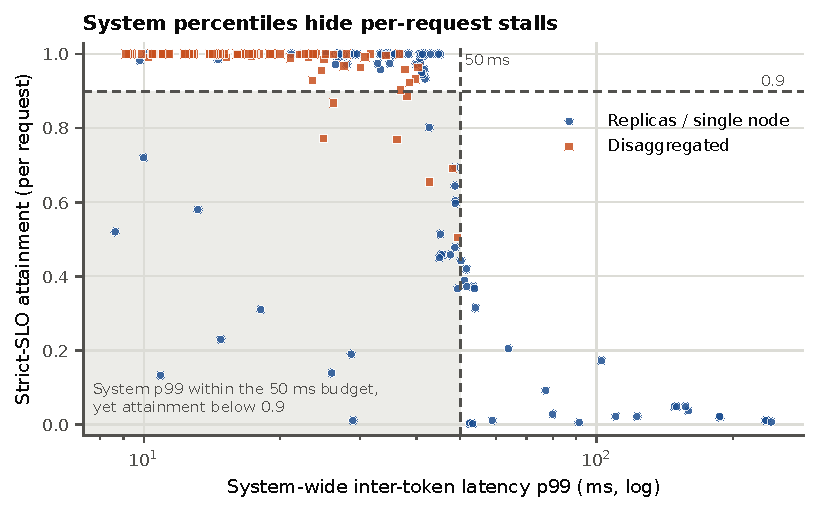
\includegraphics[width=0.82\linewidth]{fig01_request_vs_system.pdf}
\caption{System-wide inter-token latency p99 (log scale) against per-request strict-SLO attainment for the 215 runs (212 audited, 3 caution) with TTFT p99 below 1~s. The shaded region holds runs whose system p99 is within 50~ms yet whose attainment is below 0.9: 21 replica or single-node runs and 7 disaggregated runs.}
\label{fig:stalls}
\end{figure}

The system-wide p99 of inter-token latency pools every gap of every request, and it can look healthy while many requests still stall (Figure~\ref{fig:stalls}). Of the 215 runs with TTFT p99 below 1~s, 28 had system p99 at or below 50~ms but attainment below 0.9. For example, two g7e replicas serving 26B FP8 with 4K inputs at 0.25 requests/s per GPU had a system p99 of 8.6~ms, yet 48\% of requests had at least one gap over 50~ms. All later verdicts are per request.

\subsection{The chunk size sets the replicas' stall}\label{sec:chunk}

\begin{figure}[!htbp]
\centering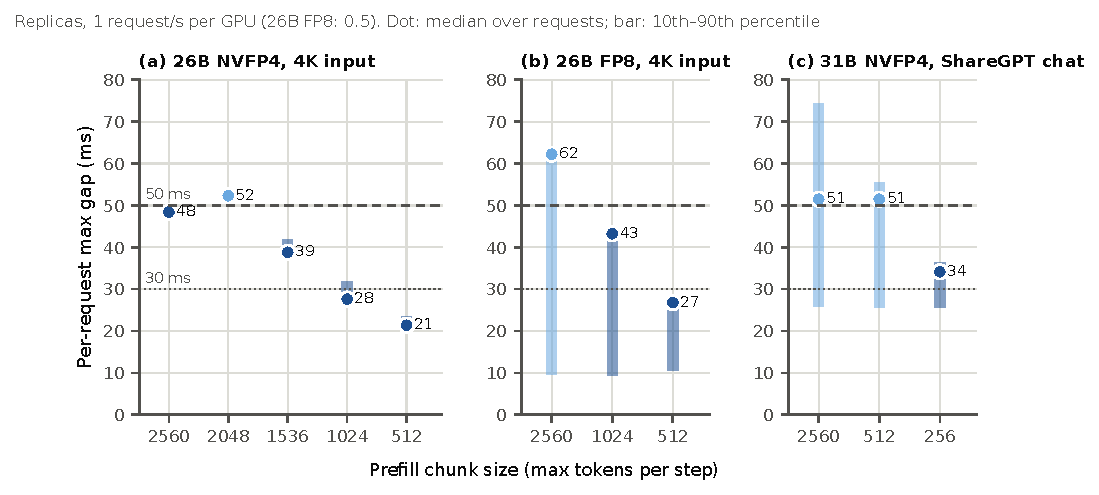
\includegraphics[width=\linewidth]{v1_chunk_stall.pdf}
\caption{Per-request longest gap of colocated replicas by chunk size (two g7e nodes in a placement group). Dot: median over requests; bar: 10th--90th percentile; light dots have a median above 50~ms; dashed and dotted lines mark 50 and 30~ms. (a) 26B NVFP4, 4K input, 1 request/s per GPU. (b) 26B FP8, 4K input, 0.5 requests/s per GPU. (c) 31B NVFP4, ShareGPT chat, 1 request/s per GPU. The 2,560-token points pool the repeats of sessions E5, E7, and E8.}
\label{fig:chunk}
\end{figure}

A replica stalls when another request's prefill joins the step, and the stall lasts as long as that step. With 4K inputs and 512 outputs almost every request overlaps another request's prefill, so its longest gap is roughly the time of a step that carries a full chunk. For 26B NVFP4 that time fell with the chunk (Figure~\ref{fig:chunk}a): the median longest gap was 48.4~ms at 2,560 tokens, 38.8~ms at 1,536, 27.6~ms at 1,024, and 21.4~ms at 512, while median TTFT rose from 132 to 205~ms. Between 1,024 and 2,048 tokens the step grew by about 24~\textmu s per token; below 1,024 it shrank more slowly toward the decode-only step, about 9~ms at this load. The 2,560-token median sat 1.6~ms under the 50~ms limit, so the replicas' verdicts at that chunk hinged on a small margin. A 2,048-token chunk gave 52.3~ms, longer than 2,560; we could not tell whether the even split of a 4K input into two 2,048-token pieces or the different multimodal setting of the 2,560 control causes this.

Heavier FP8 weights make each step longer: at 0.5 requests/s per GPU the median longest gap was 62, 43, and 27~ms at 2,560, 1,024, and 512 tokens, with attainment 0.13, 0.99, and 1.00 (Figure~\ref{fig:chunk}b). For 31B chat the longest gap depends on the longest prompt prefilled on the same replica while a request decodes (Figure~\ref{fig:chunk}c). In 2,560-token runs at 1 request/s per GPU, 99--100\% of requests kept every gap under 50~ms when that prompt had fewer than 200 tokens, 43\% with 200--400 tokens, 12\% with 400--800, and none above 800. A 512-token chunk therefore did not help (attainment 0.44, the same as 2,560), and a 256-token chunk did (1.00 in two runs, median longest gap 34~ms, TTFT unchanged at 79~ms).

\subsection{Head to head at equal GPU count}\label{sec:h2h}

\begin{figure}[!htbp]
\centering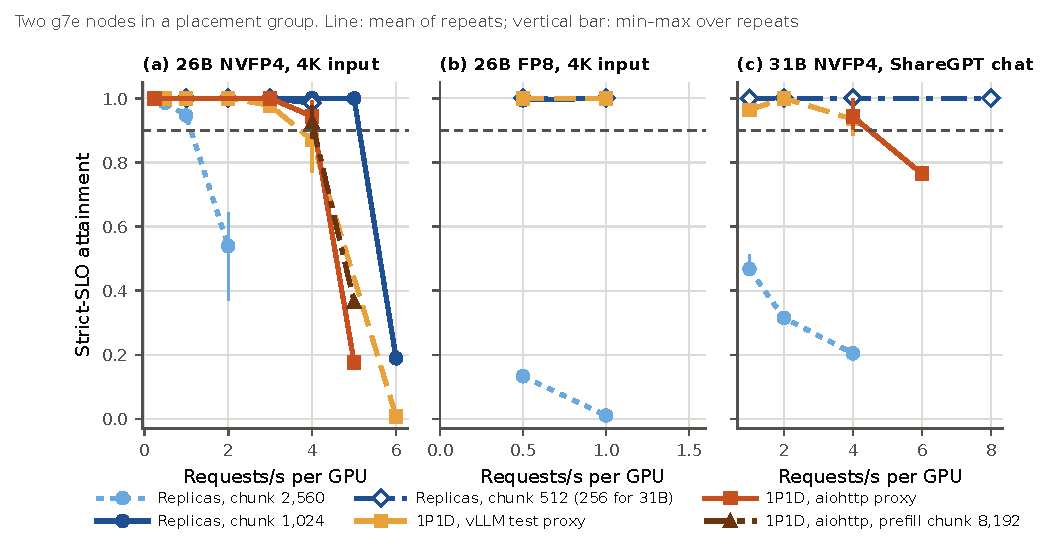
\includegraphics[width=\linewidth]{v1_head_to_head.pdf}
\caption{Strict-SLO attainment against load on two g7e nodes in a placement group. Blue: replicas at the chunk shown (runs that reached the proxy's connection cap are excluded; the 1,024-token points at 4 requests/s per GPU and above come from E9). Orange and brown: 1P1D with vLLM's test proxy (light, dashed), our aiohttp proxy (dark, solid), or our aiohttp proxy with an 8,192-token prefill chunk (brown). Lines connect the mean of repeats; vertical bars span the minimum and maximum. The dashed horizontal line is 0.9. The 2,048- and 1,536-token replicas are omitted for readability.}
\label{fig:h2h}
\end{figure}

\begin{table}[!htbp]
\centering\small
\begin{tabularx}{\linewidth}{lLLL}
\toprule
Workload & Replicas, chunk 2,560 & Replicas, best chunk & 1P1D \\
\midrule
26B NVFP4, 4K & 1 req/s, \$2.00, 132~ms & 5 (1,024), \$0.38, 259--278~ms & 3, \$0.63, 366~ms (borderline at 4) \\
26B FP8, 4K & none & $\ge$1 (512 or 1,024), $\le$\$1.87 & $\ge$1, $\le$\$1.89 \\
31B NVFP4, chat & none & $\ge$8 (256), $\le$\$0.67, 117~ms & 4, \$1.67, 304~ms \\
\bottomrule
\end{tabularx}
\caption{Supported load under the strict SLO (requests/s per GPU; every repeat $\ge$0.9), cost per million SLO-meeting output tokens at that load (g7e, \$3.363 per GPU-hour, client excluded), and median TTFT at that load. ``$\ge$'' and ``$\le$'': the configuration still passed at the highest rate we measured.}
\label{tab:cost}
\end{table}

Measured against replicas at a 2,560-token chunk, disaggregation looked decisive (Figure~\ref{fig:h2h}, dotted lines). For 26B with 4K inputs, replicas passed 1 request/s per GPU and failed at 2 (0.37--0.64 in five runs), while 1P1D passed 3; the cost per SLO-meeting token was \$2.00 against \$0.63 (Table~\ref{tab:cost}). For 26B FP8 and for 31B chat, only 1P1D met the strict SLO at any measured load.

Measured against replicas at a tuned chunk, the result reverses. For 26B with 4K inputs, 1,024-token replicas without the proxy cap passed 4 requests/s per GPU in three of three runs (1.000 each) and 5 in two of two (0.999 and 1.000), and collapsed at 6 (0.19). 512-token replicas passed 1--4 (0.985 at 4). 1P1D passed 3 and was borderline at 4: 0.885, 0.954, and 0.992 with our aiohttp proxy (interval 0.873--0.992) and 0.77--0.98 with the test proxy; at 5 it collapsed to 0.18 as prefills queued and gaps grew. Raising the prefill chunk to 8,192 tokens cut 1P1D's median TTFT at 4 requests/s per GPU from about 500 to 416--451~ms but did not change the verdicts (0.874 and 0.976 at 4, 0.365 at 5). Part of 1P1D's gap cost is structural: at equal GPU count its decode node carries the decodes of both GPUs' requests, and its median inter-token latency was 15.5 against 13.2~ms at 3 requests/s per GPU and 20.8 against 15.9~ms at 4. For 26B FP8, 512- and 1,024-token replicas and 1P1D all passed the highest load we measured, 1 request/s per GPU. For 31B chat, 256-token replicas passed every measured load up to 8 requests/s per GPU (1.000 at 8), while 1P1D passed 4 (0.903, 0.924, and 1.000 in three runs with our aiohttp proxy; 0.885--0.963 in four runs with the test proxy) and failed at 6 (0.765). At every load where both passed, tuned replicas reached the first token sooner (medians of 79--359~ms across chunks and loads, against 260--526~ms for 1P1D).

\subsection{Where each approach wins}\label{sec:who}

\begin{figure}[!htbp]
\centering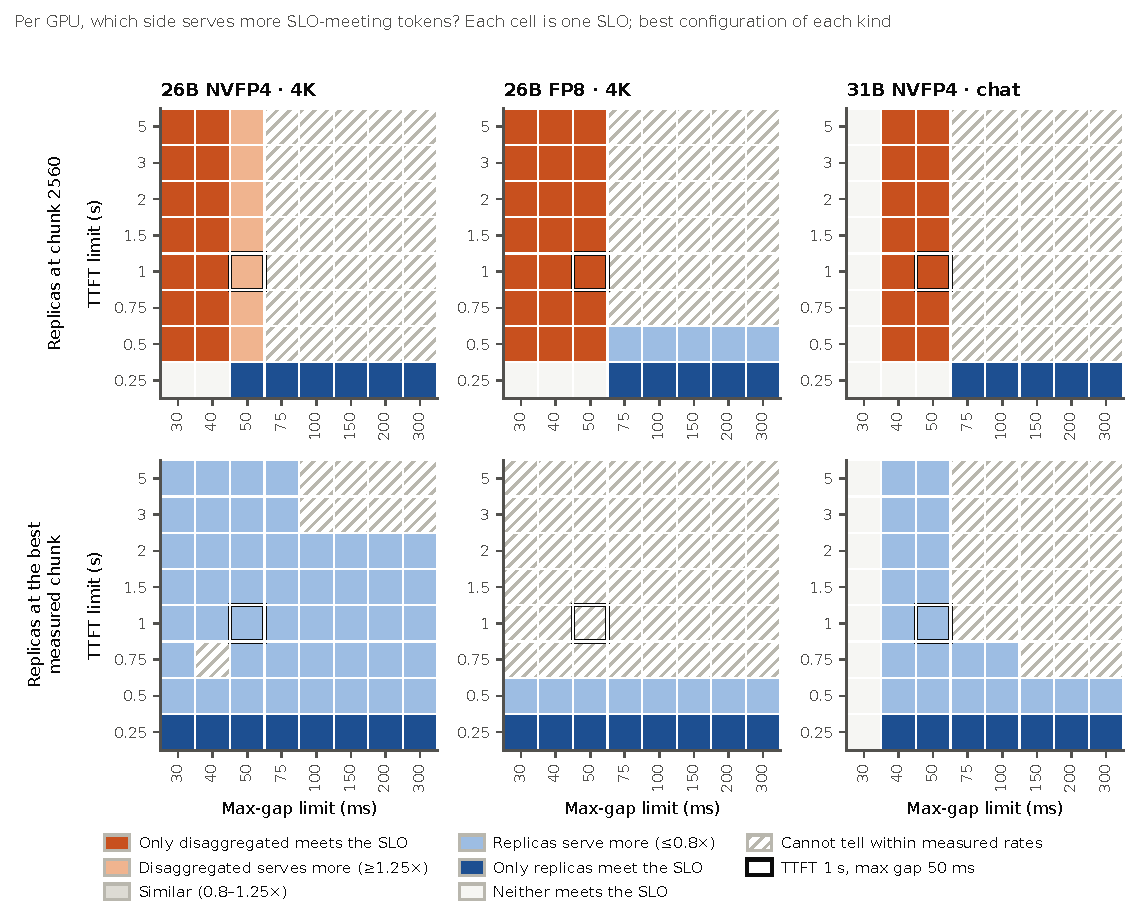
\includegraphics[width=\linewidth]{v1_who_wins.pdf}
\caption{Which approach serves more SLO-meeting tokens per GPU as the SLO changes. Each cell is one SLO (vertical: TTFT limit; horizontal: longest-gap limit), judged at the highest rate where every repeat reaches 0.9 and with the best configuration of each kind. Top row: replicas restricted to a 2,560-token chunk. Bottom row: replicas at any chunk we measured (512--2,560 for 26B, 256--2,560 for 31B). Hatched: both sides still passed at their highest measured rate. The outlined cell is the strict SLO.}
\label{fig:who}
\end{figure}

Because every per-request timing is stored, we re-judged all runs over a grid of TTFT limits (0.25--5~s) and longest-gap limits (30--300~ms) and compared the best configuration of each kind (Figure~\ref{fig:who}). Against 2,560-token replicas (top row), disaggregation wins at gap limits of 40--50~ms for all three workloads and at 30~ms for the two 26B variants; at 75~ms and above most cells cannot be decided within our measured rates. Against the best measured chunk (bottom row), no cell favors disaggregation:
\begin{itemize}
  \item For 26B NVFP4, replicas serve more in every decided cell, including 30~ms, where 512-token replicas passed 3 requests/s per GPU and 1P1D passed 2.
  \item For 26B FP8, replicas serve more when TTFT must stay under 0.5~s; elsewhere both sides passed the highest load we measured (1 request/s per GPU), so the map cannot rank them. At 30~ms, 512-token replicas reached 0.958 at that load.
  \item For 31B chat, replicas serve more at 40--50~ms; at 30~ms neither side met the SLO.
  \item Replicas are the only option when TTFT must stay under 0.25~s, because disaggregation's TTFT includes an 80--300~ms transfer.
\end{itemize}
The map picks the best configuration of each kind and cannot decide cells where both sides passed our highest rate. It covers 4K and chat inputs; at 16K and longer inputs, replicas with a small chunk would need many steps per prefill, and we did not measure that regime with a tuned chunk.

\subsection{The KV transfer over TCP}\label{sec:transfer}

\begin{figure}[!htbp]
\centering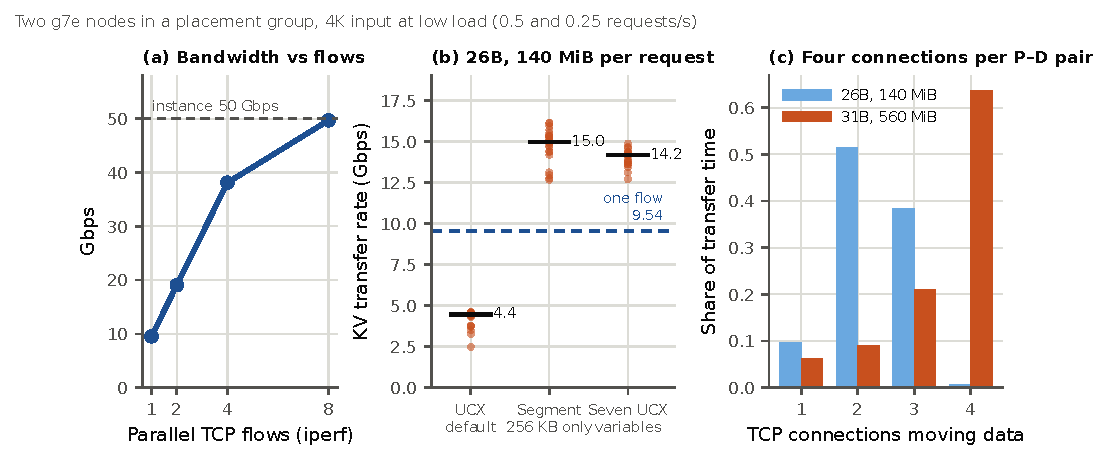
\includegraphics[width=\linewidth]{v1_transfer.pdf}
\caption{(a) Bandwidth between two g7e nodes in a placement group against the number of parallel TCP flows (iperf). (b) KV transfer rate of 26B NVFP4 (140~MiB per 4K request, 0.25 requests/s per GPU) under three UCX settings; dots are 10~s windows reported by vLLM, bars are medians, and the dashed line is one flow's limit. (c) Share of transfer time during which 1--4 TCP connections between the prefill and decode node moved data, from socket samples every 0.1~s (26B at 0.25 and 31B at 0.125 requests/s per GPU).}
\label{fig:transfer}
\end{figure}

Three things set the transfer rate: a software default, how NIXL splits a transfer, and the cloud's caps. With UCX defaults, the 8~KB TCP segment limited the transfer to a median of 4.45~Gbps, less than half of one flow's limit (Figure~\ref{fig:transfer}b). Raising only the send and receive segment sizes to 256~KB lifted it to 14.97~Gbps, a 3.4$\times$ gain. The full set of seven UCX variables gave 13.5--14.2~Gbps, 5--10\% lower: it fixes the socket buffers at 8~MB, which disables the kernel's buffer autotuning, and the sender was limited by the receive window for about 40\% of its busy time. In our first tuning session, on g7 nodes without a placement group, the seven-variable change cut median TTFT at 0.125 requests/s per GPU from 626 to 466~ms and raised attainment at 0.5 from 0.82 to 0.99.

NIXL (version 1.4.1 in vLLM v0.30.0) hands a transfer's descriptor list to up to four worker threads, each with its own UCX endpoint and TCP connection, but splits the list only when it holds at least 1,024 descriptors, in pieces of at least 1,024. A 26B 4K transfer (about 1,900--2,240 descriptors) therefore goes out in two or three pieces, a 31B 4K transfer (about 4,000--4,500) in four, and a chat-sized transfer as a single piece on a shared connection. Socket samples agree (Figure~\ref{fig:transfer}c): four connections each carried 22--27\% of the bytes and a fifth, shared one carried the rest; a 26B transfer mostly kept two or three connections busy, and a 31B transfer kept all four busy 64\% of the time.

We express the rate relative to the per-flow cap as $m = \text{effective rate} / C_{\mathrm{flow}}$. At low load $m$ was 1.4--1.6 for 26B and 1.8 for 31B. At the loads where our verdicts were decided it fell to 0.92--1.14 for 26B (3--4 requests/s per GPU), and 31B chat transfers, which are not split, reached 0.81. With all four connections busy, 31B transfers aggregated 19--21~Gbps, about half of what four iperf flows reached (38~Gbps), which points to a shared per-node limit that we did not identify. More connections alone are therefore not a sure lever.

Other settings did not help. Staging the KV cache through host memory slowed TTFT 4.7$\times$ at 0.125 requests/s per GPU on g7 and had no stable load at 0.5. Push transfer, in which the prefill node writes the KV cache, cut 31B's transfer time by 27--36\% and median TTFT by 53--62~ms but changed attainment by at most 0.04; its logged volume was 468--533~MiB per request against 560 for pull, which we could not explain. Within one node over PCIe, push has been reported about 100$\times$ faster than pull~\cite{vllm52607}; we saw no such gap across nodes. A proposed vLLM patch that overlaps the transfer with prefill layer by layer\footnote{\url{https://github.com/vllm-project/vllm/pull/56874}} supports only models with a single KV-cache group; with hybrid-attention Gemma~4 it stalled on the first request. Network credits were not a constraint: g7e.2xlarge has a fixed 50~Gbps, and on g6e.2xlarge (5~Gbps baseline, 20~Gbps burst) our 15-minute test load averaged about 1.2~Gbps, computed from the request rate and volume, below the baseline.

\subsection{The first-token cost of disaggregation}\label{sec:ttft}

\begin{figure}[!htbp]
\centering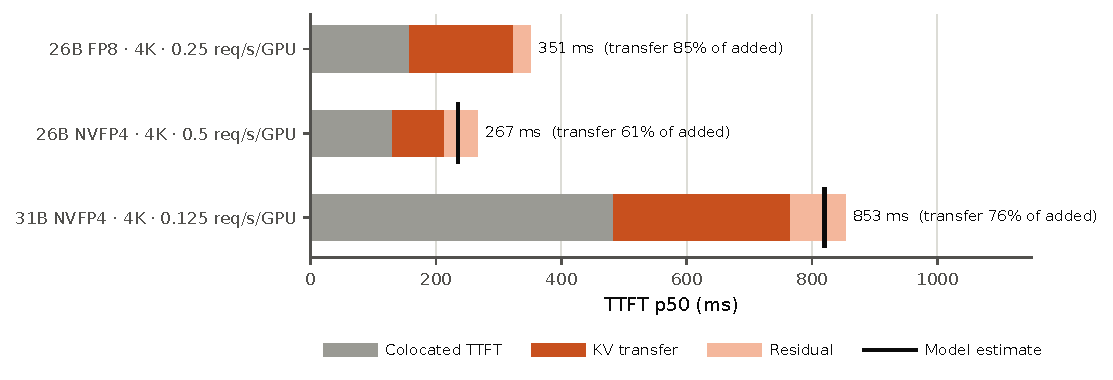
\includegraphics[width=0.92\linewidth]{v1_ttft.pdf}
\caption{Median TTFT of 1P1D split into colocated TTFT at the same load, mean KV transfer time, and residual (placement group). Black ticks are estimates from Eq.~\eqref{eq:ttft}. The first row joins measurements from two days.}
\label{fig:ttft}
\end{figure}

Disaggregation adds TTFT, and most of it is the KV transfer (Figure~\ref{fig:ttft}): 61\% of the added time for 26B NVFP4 at 0.5 requests/s per GPU (84 of 137~ms), 76\% for 31B at 0.125 (283 of 370~ms), and 85\% for 26B FP8 at 0.25. The residual, 28--87~ms, covers the decode node's first step, scheduling, and the proxy hop, and it would remain with RDMA. At low load the relation is
\begin{equation}\label{eq:ttft}
\mathrm{TTFT}_{\mathrm{PD}} \approx \mathrm{TTFT}_{\mathrm{coloc}} + \frac{V(L)}{m \times C_{\mathrm{flow}}} + \text{residual},
\end{equation}
with $V(L)$ from Eq.~\eqref{eq:vol}, $C_{\mathrm{flow}}$ the per-flow cap, and $m$ as defined above. We wrote estimates from this relation into our lab notebook before the three-node session: 235~ms for 26B at 0.5 requests/s per GPU (measured 267~ms, 14\% higher) and 810--830~ms for 31B at 0.125 (measured 853~ms); unlike the E9 predictions, these were not committed separately, so the repository cannot prove their order. The relation omits queueing: when we limited the sender's aggregate bandwidth to 1~Gbps (Appendix Figure~\ref{fig:bwsweep}), it predicted about 1.5~s against a measured 2.19~s, and an added M/D/1 waiting time is consistent with the difference (about 2.2~s). Eq.~\eqref{eq:ttft} is a low-load estimate, and $m$ falls with load. It also shows why long inputs fail: for 26B FP8 at 16K inputs, about 520~MiB take roughly 0.3--0.7~s on top of a prefill of about 0.8~s, and we measured 1P1D's TTFT 465--506~ms above the replicas', beyond a 1~s budget.

\subsection{Pitfalls: proxies that change the verdict}\label{sec:proxy}

\begin{figure}[!htbp]
\centering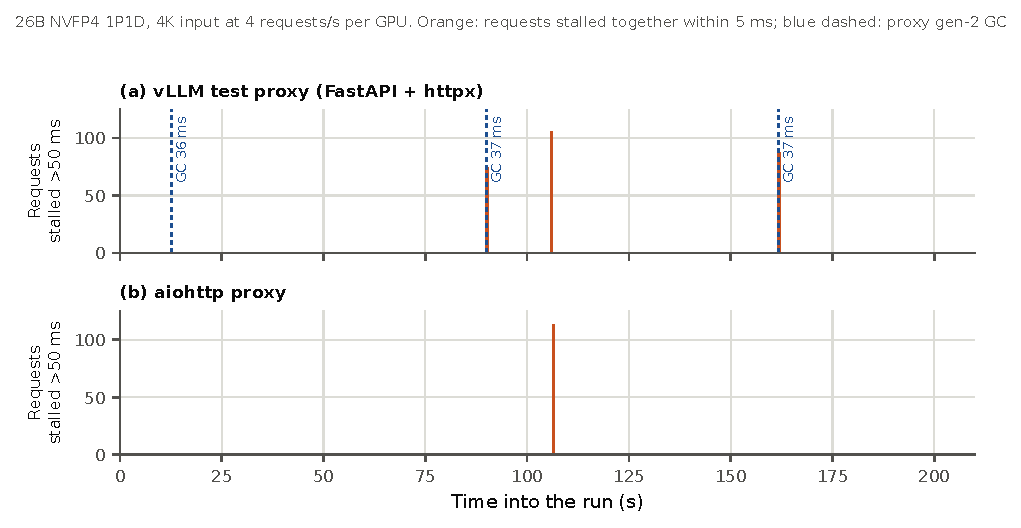
\includegraphics[width=0.9\linewidth]{v1_proxy_gc.pdf}
\caption{Global stalls in two 1P1D runs with the same seed (session E8; 26B, 4K input, 4 requests/s per GPU). Orange: number of requests whose output stream paused for more than 50~ms within the same 5~ms. Blue dashed: second-generation garbage collections in the proxy. (a) vLLM's test proxy. (b) Our aiohttp proxy.}
\label{fig:proxy}
\end{figure}

\paragraph{Garbage collection in the disaggregated proxy.} Near their limits, disaggregated runs failed in a way that 1,024-token replicas did not: one to five times per run, 40--110 in-flight requests paused together for 55--80~ms and then received a burst of tokens. In E8 we instrumented both proxies to log upstream stream gaps, event-loop lag, and garbage collection, and snapshotted the decode server's inter-token latency histogram before and after each point. For 26B 1P1D with vLLM's test proxy, four of five such events in three runs coincided within 100~ms with a second-generation garbage collection of 25--40~ms that blocked the proxy's event loop (Figure~\ref{fig:proxy}a). With our aiohttp proxy, second-generation collections took 9~ms and the loop never lagged. One event remained in three runs; the proxy received it from upstream, the decode server logged it as 113 gaps over 50~ms, and it appears at the same time in the test-proxy run with the same seed, so it is a server-side pause tied to the request sequence. For 31B chat, the events with our aiohttp proxy were also server-side: the decode server logged 110 and 316 gaps over 50~ms, and the proxy showed no collection or lag. We instrumented only session E8, so we do not attribute earlier disaggregated failures, such as the three-node 2P1D collapse, to the proxy.

\paragraph{A connection limit in the replicas' proxy.} The replicas' round-robin proxy used an HTTP client whose default limit is 100 concurrent connections. At 4--6 requests/s per GPU in E8, every TTFT failure of 1,024-token replicas came from a request that arrived while 100 or more requests were in flight (33 of 33 at 4, 393 of 393 at 5), and no request failed on gaps at 5. With the limit removed in E9, the same configuration reached 1.000 at 4 and 0.999--1.000 at 5. The cap had lowered the replicas' supported load by one step and inflated their TTFT tail.

\subsection{Other observations}\label{sec:other}
These results come from sessions before E8 and used 2,560-token replicas and the capped proxy; we report them with those caveats.
\begin{itemize}
  \item \textbf{Three nodes} (Appendix Figures~\ref{fig:scale26} and~\ref{fig:scale31}). Neither 1P2D nor 2P1D exceeded 1P1D per GPU for 26B with 4K inputs (1P2D: 0.906 at 3 requests/s per GPU; 2P1D: 0.77), and three 2,560-token replicas passed 1 request/s per GPU. We draw no rule for the prefill-to-decode ratio. For 31B with 4K inputs no configuration held a 1~s TTFT reliably: a 4K prefill takes about 480~ms and the transfer about 280~ms.
  \item \textbf{Input length} (g7, before transfer tuning; Appendix Figure~\ref{fig:inputlen}). At 0.25 requests/s per GPU with 4K inputs, 1P1D reached 0.96 and replicas 0.23. At 16K, prefill alone pushed the replicas' TTFT over 1~s and the transfer pushed 1P1D's over, so neither met the strict SLO; under the relaxed SLO 1P1D reached 0.47 and replicas 0.17. At 32K all failed.
  \item \textbf{Weight precision} (g7e, same day; Appendix Figure~\ref{fig:quant}). At 0.5 requests/s per GPU with 4K inputs, 2,560-token replicas reached 0.97 (NVFP4), 0.13 (FP8), and 0.03 (BF16), and 1P1D 1.00 in all three. Section~\ref{sec:chunk} shows that a 512- or 1,024-token chunk rescues FP8.
  \item \textbf{Real trace} (Appendix Figure~\ref{fig:trace}). Replaying the Azure conversation trace, all 26B configurations passed (4 and 5.9 requests/s in total); 1P1D's TTFT was about 120~ms higher. For 31B at 3.7 requests/s in total, both failed: 2,560-token replicas on gaps (0.05) and 1P1D on the TTFT tail (0.28).
  \item \textbf{Other GPUs and push transfer} (Appendix Figures~\ref{fig:gpuspeed} and~\ref{fig:push}) behaved as in the main results; repeat stability is in Appendix Figure~\ref{fig:repeat}, and practical pitfalls are listed in Appendix~\ref{app:pitfalls}.
  \item \textbf{Correctness.} With greedy decoding and Gemma's chat template, disaggregated 31B gave the same answers as a single node; long outputs diverged only in late, near-tied tokens (30--160 characters in), and push matched pull byte for byte on 8 of 8 prompts after a restart. 26B was not deterministic even on a single node, so we used a gate (short outputs byte-identical; long outputs sharing at least 40\% of words of five or more letters, calibrated at $\ge$0.58 for true pairs and $\le$0.17 for swapped prompts); all disaggregated outputs passed.
\end{itemize}

\section{Discussion}

\subsection{Answers to the research questions}

\paragraph{RQ1.} The chunk size. In our 4K workload a replica's longest gap was roughly the time of a step carrying a full chunk of another request's prefill; in chat traffic it followed the longest prompt prefilled alongside. For 26B, the median longest gap fell from 48 to 21~ms as the chunk shrank from 2,560 to 512 tokens, at a TTFT cost of about 70~ms and without losing supported load down to 1,024 tokens. For dense 31B chat the chunk had to be small (256 tokens).

\paragraph{RQ2.} The KV transfer, about 61--85\% of the added TTFT at low load. Its time is the KV volume of Eq.~\eqref{eq:vol} divided by the effective bandwidth, which the UCX segment size limits first and the per-flow cap and NIXL's splitting limit next (Eq.~\eqref{eq:ttft}). Queueing adds to it under load, and the decode node's doubled batch adds to the gaps.

\paragraph{RQ3.} In our measurements, only when the chunk could not be reduced. Against replicas held at a 2,560-token chunk, near the minimum vLLM imposes on Gemma~4 with video input enabled, disaggregation over TCP served about 3$\times$ more at 50~ms. Against replicas at a 256--1,024-token chunk, it served no more in any SLO we tested, down to 30~ms, and always reached the first token later. Disaggregation might still win where no acceptable chunk meets the gap limit, for example at gap limits below what the smallest workable chunk reaches or with very long inputs, which we did not measure.

\subsection{A procedure before disaggregating over TCP}
\begin{enumerate}
  \item \textbf{Measure the replicas' longest gap per request, not system percentiles.} With long inputs it approaches the time of a step carrying one full chunk; with chat it follows the longest co-scheduled prompt.
  \item \textbf{Shrink the chunk until that gap fits the limit.} Check that the stack allows it (for Gemma~4 in vLLM v0.30.0, disable every modality) and that TTFT and throughput remain acceptable; in our runs 512--1,024 tokens (26B) and 256 tokens (31B chat) cost at most about 80~ms of median TTFT and no supported load.
  \item \textbf{Disaggregate only if no acceptable chunk fits}, and check that the transfer fits the TTFT budget with Eq.~\eqref{eq:ttft}: KV volume from Eq.~\eqref{eq:vol}, per-flow cap from one iperf flow, and $m$ measured at the target load (it fell to about 1 in our runs).
  \item \textbf{Fix the serving path}: raise UCX's TCP segment size (send and receive together, without pinning socket buffers), keep nodes in a placement group, and use proxies that neither cap connections nor pause for garbage collection.
\end{enumerate}

\subsection{RDMA, EFA, and scope}
EFA is available on the 8xlarge sizes of the same instance families, without GPUDirect RDMA on g6e and g7e~\cite{awsefa}, at roughly 1.6--2$\times$ the hourly price according to a third-party listing~\cite{vantage}. Those sizes also have four times the vCPUs, and NIXL would use EFA through libfabric rather than UCX over TCP, so the comparison would change more than the network. EFA would shrink the transfer term of Eq.~\eqref{eq:ttft}, but not the residual, the decode node's doubled batch, or the replicas' chunk trade-off. We did not measure EFA. The per-flow cap is an AWS policy, and NIXL's splitting rule belongs to one version; on other clouds and versions, measure one flow and several flows with iperf first.

\section{Limitations}
\begin{itemize}
  \item One model family (Gemma~4) with hybrid attention; models with only global attention have larger KV caches.
  \item One vLLM version (v0.30.0), one AWS availability zone, at most three nodes, and no RDMA or EFA baseline.
  \item We measured chunks down to 512 tokens for 26B and 256 for 31B, and inputs up to 4K with tuned chunks; longer inputs and tighter gap limits with small chunks were not measured.
  \item Decisive points have one to three runs, and rates are resolved to 1 request/s per GPU; several verdicts are bounded by our highest measured rate.
  \item The disaggregated side kept most defaults (decode node limited to 256 sequences, NIXL's four threads; the prefill chunk was varied once).
  \item Sessions before E9 used a replica proxy capped at 100 connections; we excluded the 9 runs that reached the cap, but results from earlier sessions still used 2,560-token replicas.
  \item No prompt reuse; prefix-cache hits would shorten prefills and transfers. Latency was measured at the client and includes the proxy.
  \item The 2,560-token replica controls had a different multimodal setting from the smaller chunks; some comparisons join sessions from different days, and sessions before E7 used a smaller client instance.
\end{itemize}

\section{Conclusion}
Over TCP between rented single-GPU nodes, disaggregation works: once UCX's segment size is raised, its first-token cost is mostly a KV transfer that can be estimated before deployment. Its benefit, keeping other requests' prefills out of the decode steps, is also what chunked prefill provides. Against replicas held at a 2,560-token chunk, disaggregation served about three times more under a 50~ms gap limit; against replicas with a 256--1,024-token chunk, it served no more under any SLO we tested and always delivered the first token later. Choose the chunk first, and disaggregate over TCP when the chunk cannot be made small enough.

\section*{Use of AI tools}
An AI coding assistant (Claude) was used to write measurement and analysis scripts, operate the cloud infrastructure, run two mock peer reviews that prompted sessions E8 and E9, draft figures, and draft and translate the text. All experiments ran on real hardware, and the author checked the reported numbers against the raw data.

\section*{Acknowledgments}
This work was carried out at the author's own expense, about \$270 of cloud usage.

\bibliographystyle{unsrtnat}
\bibliography{refs}

\clearpage
\appendix
\setcounter{figure}{0}
\renewcommand{\thefigure}{A\arabic{figure}}
\section{Additional figures}
These figures come from sessions before E8 and use 2,560-token replicas. Rates printed inside them are totals for two GPUs unless the axis says per GPU; the captions give per-GPU rates.

\begin{figure}[H]
\centering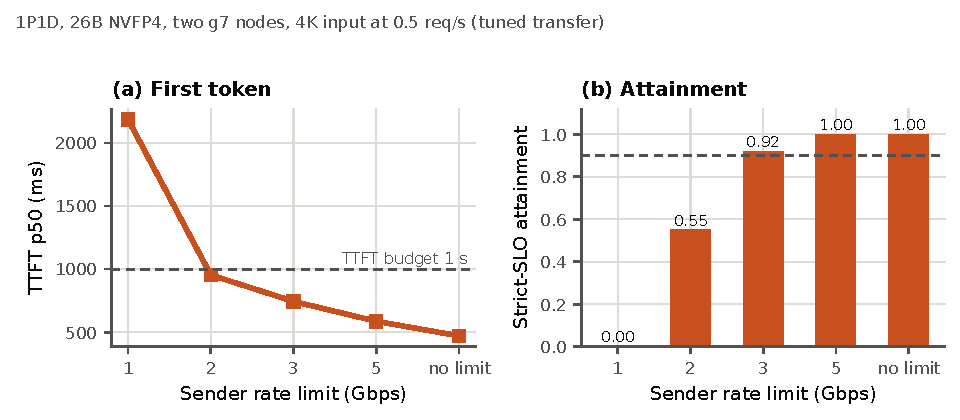
\includegraphics[width=0.8\linewidth]{fig02_bandwidth_sweep.pdf}
\caption{1P1D on two g7 nodes, 26B NVFP4, 4K input at 0.25 requests/s per GPU, with the sender's aggregate bandwidth limited by a token-bucket filter. (a) Median TTFT. (b) Strict-SLO attainment. After transfer tuning.}
\label{fig:bwsweep}
\end{figure}

\begin{figure}[H]
\centering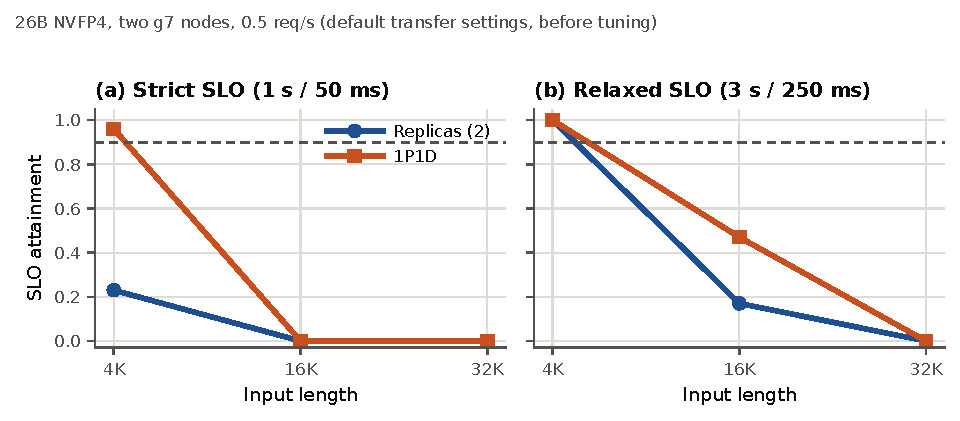
\includegraphics[width=0.8\linewidth]{fig05_input_length.pdf}
\caption{Attainment by input length on two g7 nodes, 26B NVFP4, 0.25 requests/s per GPU, before transfer tuning. (a) Strict SLO. (b) Relaxed SLO.}
\label{fig:inputlen}
\end{figure}

\begin{figure}[H]
\centering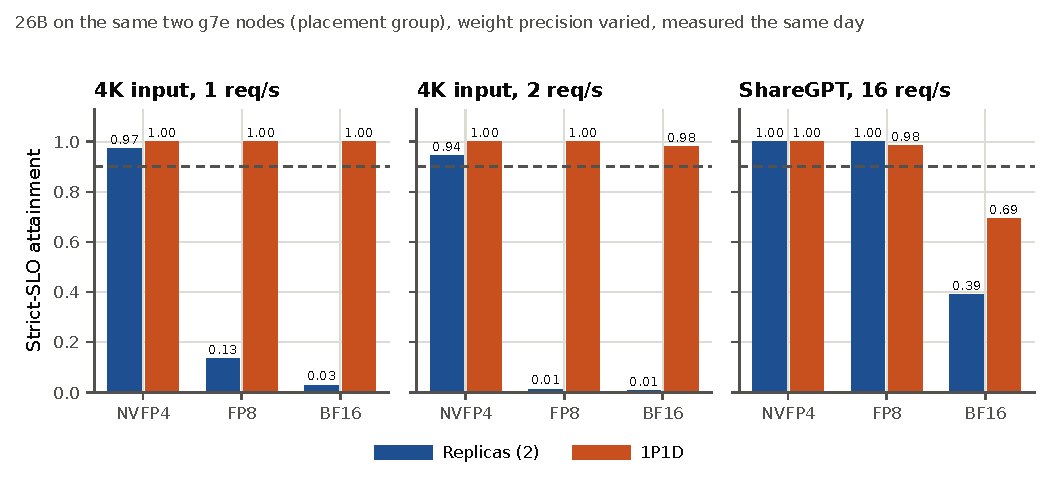
\includegraphics[width=0.85\linewidth]{fig10_quantization.pdf}
\caption{Weight precision varied on the same two g7e nodes in a placement group, 26B, same day, 2,560-token replicas. Panel titles give total rates (0.5 and 1 request/s per GPU for 4K input, 8 for ShareGPT).}
\label{fig:quant}
\end{figure}

\begin{figure}[H]
\centering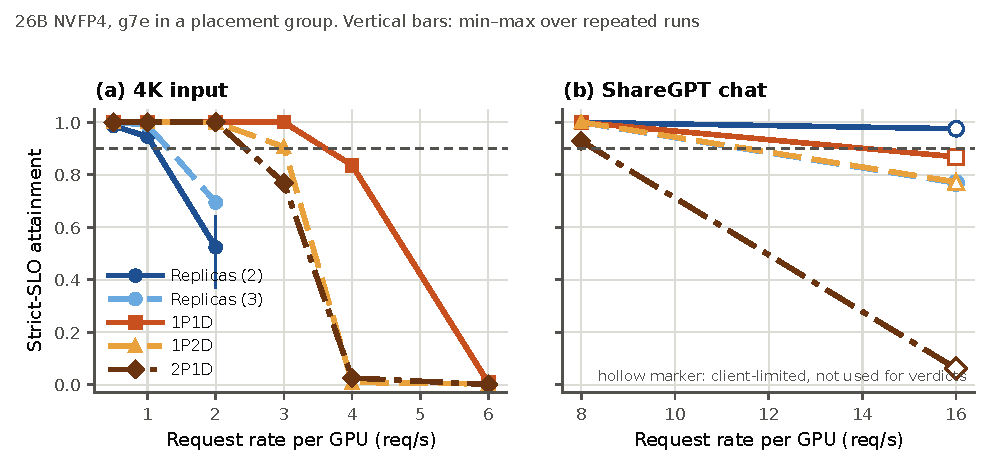
\includegraphics[width=0.9\linewidth]{fig08_scaling_26b.pdf}
\caption{26B NVFP4 on g7e in a placement group with two and three nodes (sessions E5 and E7, test proxy, 2,560-token replicas). (a) 4K input. (b) ShareGPT chat; hollow markers are client-limited.}
\label{fig:scale26}
\end{figure}

\begin{figure}[H]
\centering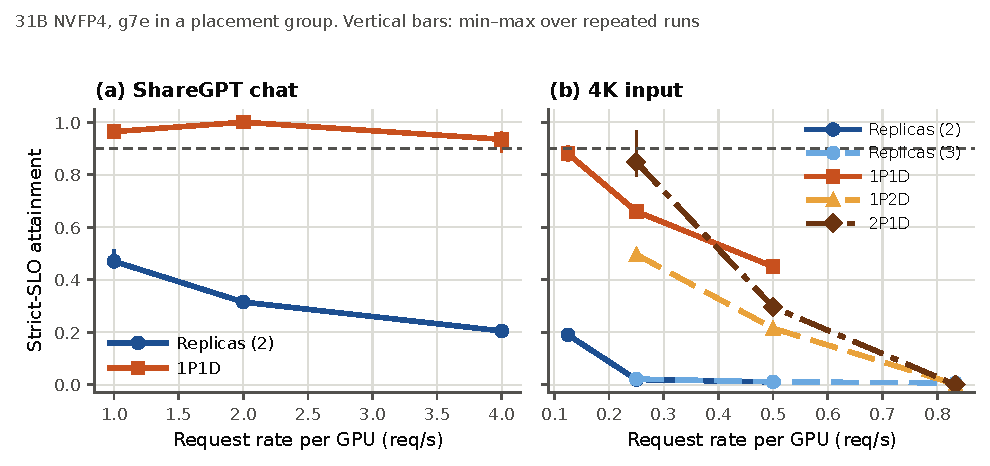
\includegraphics[width=0.9\linewidth]{fig09_scaling_31b.pdf}
\caption{31B NVFP4 on g7e in a placement group with two and three nodes (sessions E5 and E7). (a) ShareGPT chat. (b) 4K input.}
\label{fig:scale31}
\end{figure}

\begin{figure}[H]
\centering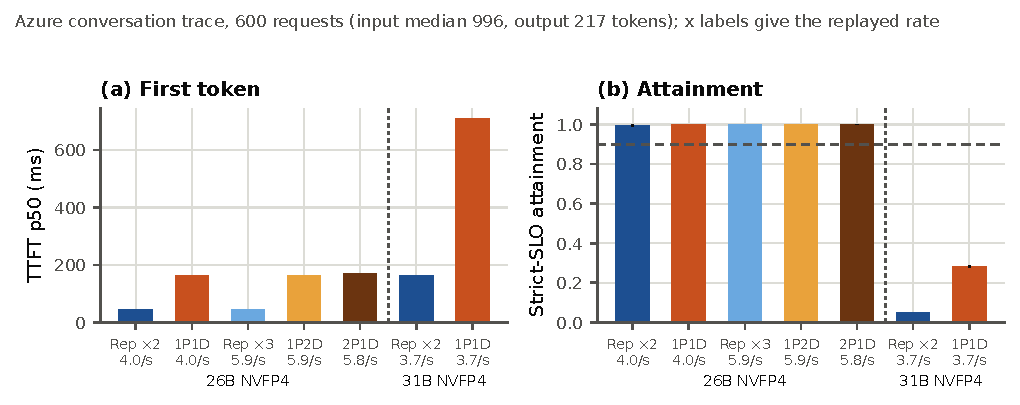
\includegraphics[width=0.85\linewidth]{fig11_trace.pdf}
\caption{Azure conversation trace, 600 requests. (a) Median TTFT. (b) Strict-SLO attainment. Numbers under the axis give the replayed total rate; left of the dotted line is 26B, right is 31B.}
\label{fig:trace}
\end{figure}

\begin{figure}[H]
\centering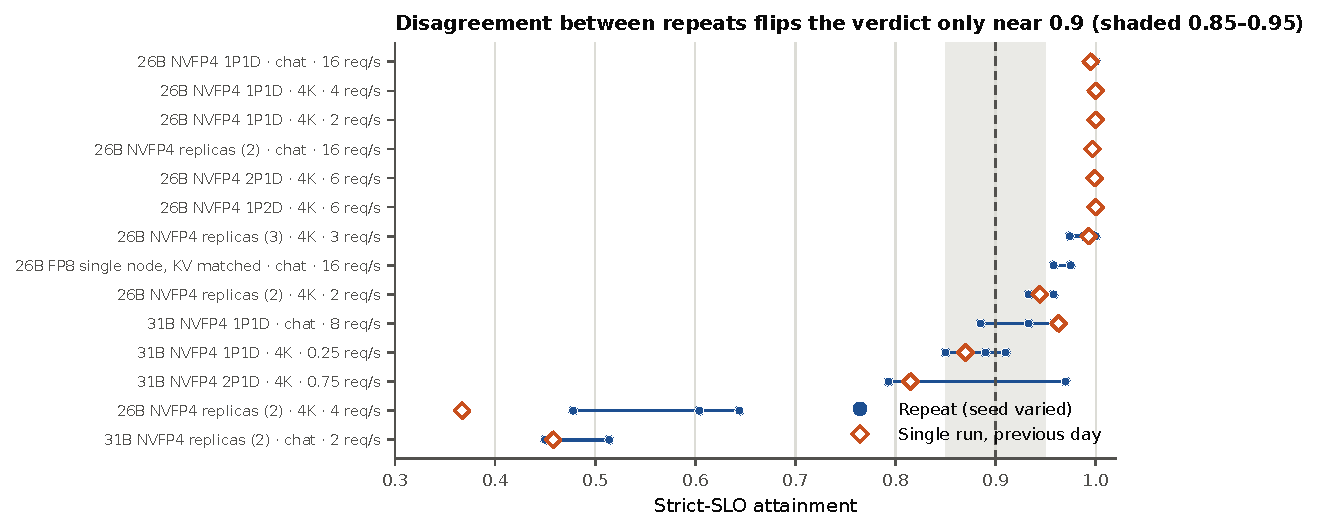
\includegraphics[width=0.85\linewidth]{fig13_repeatability.pdf}
\caption{Attainment at points measured at least three times with different seeds (session E7) and the previous day's run (E5). Row labels give total rates. The gray band is 0.85--0.95.}
\label{fig:repeat}
\end{figure}

\begin{figure}[H]
\centering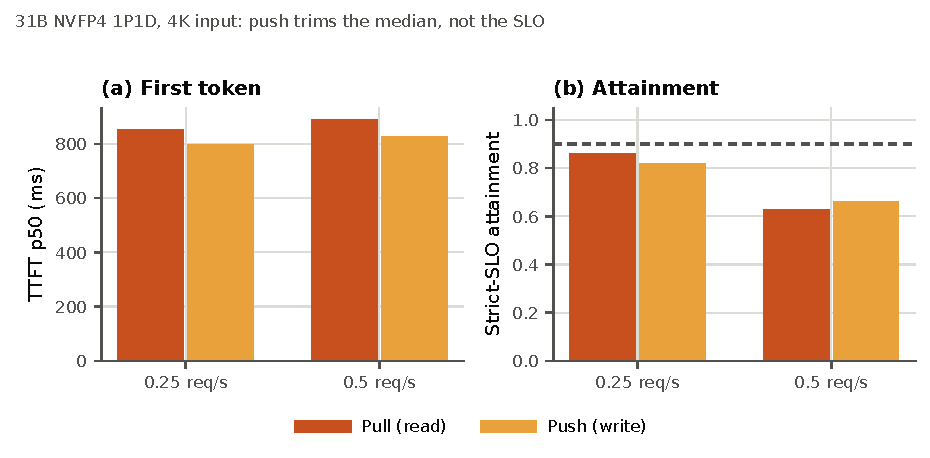
\includegraphics[width=0.8\linewidth]{fig14_push_vs_pull.pdf}
\caption{31B NVFP4 1P1D, 4K input, pull versus push transfer at 0.125 and 0.25 requests/s per GPU. (a) Median TTFT. (b) Strict-SLO attainment.}
\label{fig:push}
\end{figure}

\begin{figure}[H]
\centering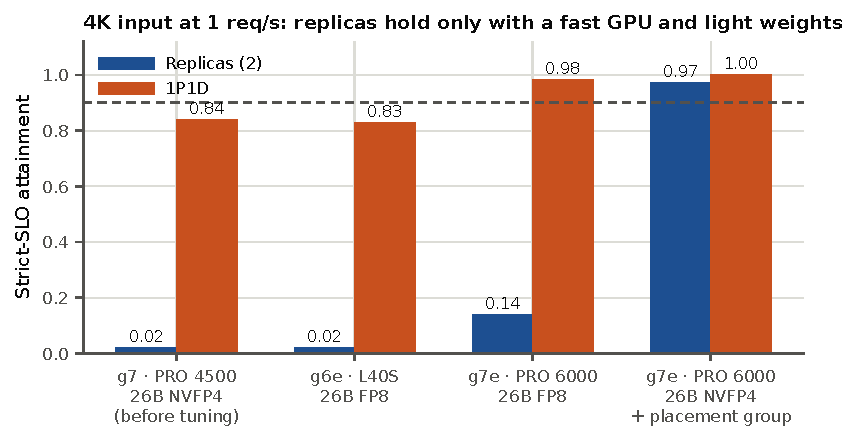
\includegraphics[width=0.85\linewidth]{fig06_gpu_speed_4k.pdf}
\caption{Strict-SLO attainment of two-node configurations at 4K input and 0.5 requests/s per GPU by GPU and precision. The g7 measurement predates transfer tuning.}
\label{fig:gpuspeed}
\end{figure}

\section{Practical pitfalls}\label{app:pitfalls}
\begin{itemize}
  \item Gemma~4 in vLLM v0.30.0 rejects chunks below 2,496 tokens unless images, audio, and video are all disabled; with all three disabled, a 2,560-token chunk fails at engine start.
  \item aiohttp's client limits a session to 100 concurrent connections by default; a proxy built on it queues requests silently beyond that.
  \item vLLM's test proxy for NIXL pauses all streams during garbage collection (Section~\ref{sec:proxy}); our aiohttp proxy had one keep-alive race in 1,440 requests.
  \item If UCX's TCP receive segment is smaller than the send segment, the engine refuses to start; raise both. Pinning socket buffers disables kernel autotuning.
  \item At high rates the proxy hit the operating system's file-handle limit (1,024 by default); a disaggregated proxy opens two connections per request and hits it sooner.
  \item Trace replay in vLLM v0.30.0 without an explicit request count builds an empty request list.
  \item Replaying the same seeded requests against a server with prefix caching enabled makes later points hit the cache.
  \item New cloud workspaces create separate security groups; the client needs an explicit ingress rule to reach new nodes. Cluster placement groups may take 15--45 minutes to find capacity for a second node.
\end{itemize}

\section{UCX settings}\label{app:ucx}
The tuned set used in sessions E4--E9:
{\small
\begin{itemize}
  \item \texttt{UCX\_TCP\_TX\_SEG\_SIZE=256k}, \texttt{UCX\_TCP\_RX\_SEG\_SIZE=256k}
  \item \texttt{UCX\_TCP\_MAX\_IOV=16}, \texttt{UCX\_TCP\_MAX\_POLL=-1}
  \item \texttt{UCX\_TCP\_SNDBUF=8m}, \texttt{UCX\_TCP\_RCVBUF=8m}
  \item \texttt{UCX\_RNDV\_FRAG\_SIZE=host:4M,cuda:8M}
  \item with \texttt{UCX\_TLS=tcp,cuda\_copy,cuda\_ipc} and \texttt{UCX\_NET\_DEVICES=all} in every disaggregated run
\end{itemize}}
Session E8 showed that the two segment sizes alone give a slightly higher rate (Section~\ref{sec:transfer}). We did not change kernel socket limits, so the fixed 8~MB buffers were capped by the kernel's maximums.

\section{Deviations from the pre-registered protocol}\label{app:dev}
\begin{itemize}
  \item Gap limit: five times each model's decode step became a common 50~ms (Section~\ref{sec:slo}). One-token outputs pass the gap criterion since session E8.
  \item Chunk size: 2,048 was planned; Gemma~4 forced 2,560 until sessions E8 and E9 swept 256--2,048.
  \item Proxy: one proxy for both approaches was planned; replicas and disaggregated runs used different proxies, and the replicas' proxy was capped at 100 connections until E9.
  \item Equivalence band: 0.9--1.1 was planned; Figure~\ref{fig:who} uses 0.8--1.25.
  \item Confidence intervals: a request-level bootstrap was planned; we report hierarchical bootstrap intervals for decisive points (Appendix~\ref{app:ci}).
  \item Client: a fixed c6i.2xlarge was planned; sessions before E7 used c6i.xlarge. Warm-up was implemented from E7 on.
  \item Reference points on H100 and on a two-GPU g5 node were not measured.
  \item Session E9's predictions were committed before the session (repository commit \texttt{8775497}); four of five held, and the fifth (1P1D with an 8,192-token prefill chunk passing 4 requests/s per GPU) did not (0.874 and 0.976).
\end{itemize}

\section{Decisive points}\label{app:ci}
\setcounter{table}{0}
\renewcommand{\thetable}{F\arabic{table}}
\begin{table}[H]
\centering\footnotesize
\begin{tabularx}{\linewidth}{Lllll}
\toprule
Point & per GPU & gap limit & runs & attainment (each run), 95\% interval \\
\midrule
26B 4K, replicas chunk 1,024 (E9) & 4 & 50~ms & 3 & 1.000, 1.000, 1.000; 1.000--1.000 \\
26B 4K, replicas chunk 1,024 (E9) & 5 & 50~ms & 2 & 0.999, 1.000; 0.998--1.000 \\
26B 4K, replicas chunk 512 (E9) & 4 & 50~ms & 1 & 0.985; 0.965--0.999 \\
26B 4K, 1P1D aiohttp (E8) & 4 & 50~ms & 3 & 0.954, 0.992, 0.885; 0.873--0.992 \\
26B 4K, 1P1D test proxy (E5--E8) & 4 & 50~ms & 4 & 0.836, 0.900, 0.975, 0.767; 0.774--0.953 \\
26B 4K, 1P1D, prefill chunk 8,192 (E9) & 4 & 50~ms & 2 & 0.874, 0.976; 0.827--0.988 \\
26B 4K, replicas chunk 512 (E9) & 2 & 30~ms & 2 & 1.000, 1.000; 1.000--1.000 \\
26B 4K, 1P1D test proxy (E5, E7) & 2 & 30~ms & 4 & 0.954, 1.000, 0.919, 0.958; 0.912--0.993 \\
26B FP8 4K, replicas chunk 512 (E9) & 1 & 30~ms & 1 & 0.958; 0.900--1.000 \\
26B FP8 4K, 1P1D test proxy (E7) & 1 & 30~ms & 1 & 1.000; 1.000--1.000 \\
31B chat, replicas chunk 256 (E9) & 8 & 50~ms & 1 & 1.000; 1.000--1.000 \\
31B chat, 1P1D aiohttp (E8, E9) & 4 & 50~ms & 3 & 0.924, 0.903, 1.000; 0.887--1.000 \\
31B chat, 1P1D test proxy (E5, E7) & 4 & 50~ms & 4 & 0.963, 0.933, 0.958, 0.885; 0.888--0.970 \\
31B chat, 1P1D aiohttp (E9) & 6 & 50~ms & 1 & 0.765; 0.666--0.855 \\
\bottomrule
\end{tabularx}
\caption{Strict-SLO attainment (TTFT $\le$1~s) at the points that decide the comparisons, with 95\% intervals from a hierarchical bootstrap (resample runs, then 20 time blocks within each run). Script: \texttt{harness/decisive\_ci.py}.}
\label{tab:ci}
\end{table}

\section{Data and code}\label{app:data}
We release the measurement harness, configurations, analysis scripts, both mock reviews with their scripts, and per-request raw data \todo{GitHub URL and Zenodo DOI}. Raw data are stored per session (\texttt{results/\textless session\textgreater/}).

\setcounter{table}{0}
\renewcommand{\thetable}{G\arabic{table}}
\begin{table}[H]
\centering\footnotesize
\begin{tabularx}{\linewidth}{llllL}
\toprule
Session & Date (UTC) & Instances & Models & Main content \\
\midrule
B  & 2026-09-25 & 2$\times$g7 & 26B NVFP4 & input-length grid \\
D  & 2026-09-26 & 2$\times$g7 & 26B NVFP4 & transfer tuning, bandwidth limit \\
E1 & 2026-09-26 & g6e, g7e & 26B FP8, 31B FP8 & cross-GPU, KV matching \\
E2 & 2026-09-26 & 2$\times$g7e & 26B FP8 & two-node comparison, 16K \\
E3 & 2026-09-27 & 2$\times$g6e & 26B FP8 & L40S pair, network credits \\
E4 & 2026-09-27 & 2$\times$g7e, PG & 26B FP8 & placement group, transfer settings \\
E5 & 2026-09-27 & 2--3$\times$g7e, PG & 26B, 31B NVFP4 & scaling, transfer estimates \\
E6 & 2026-09-27 & 2$\times$g7e, PG & 26B, 31B NVFP4 & push transfer, correctness \\
E7 & 2026-09-28 & 2--3$\times$g7e, PG & 26B (3 precisions), 31B & repeats, trace, precision \\
E8 & 2026-09-29/30 & 2$\times$g7e, PG & 26B NVFP4/FP8, 31B & chunk sweep, proxy instrumentation, socket counts, UCX ablation \\
E9 & 2026-09-30 & 2$\times$g7e, PG & 26B NVFP4/FP8, 31B & 512-token chunk, uncapped replica proxy, prefill chunk 8,192, 31B limits \\
\bottomrule
\end{tabularx}
\caption{Measurement sessions (PG: cluster placement group). Sessions A, A$'$, C1, and P are prefix-cache-contaminated or setup runs and are not used.}
\label{tab:folders}
\end{table}

\end{document}
